\section{Введение}
\label{sec:Chapter0} \index{Chapter0}
В ряде приложений возникают большие линейные системы с многими правыми частями. такую задачу можно записать в блочном виде:\\
\begin{figure}[H]
    \centering
    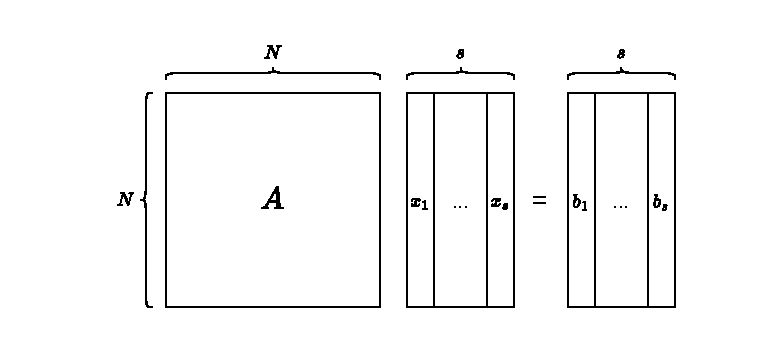
\includegraphics[width=0.5\linewidth]{images/system.pdf}
    % \caption{Caption}
    \label{fig:system}
\end{figure}
$$AX=B,$$
где $A$ - $N\times N$ невырожденная разреженная матрица системы;
$B$ - $N\times s$ невырожденная матрица, столбцы - правые части; 
$X$ - $N\times s$ матрица, столбцы - решения для соответствующих правых частей. 
Также еще предполагаем, что $s\ll N$.
Такие задачи можно решать прямыми методами, однако они не подходят для больших 
задач. Так что естественным является использование 
блочных крыловских методов.\\

\par В преимущества блочных крыловских методов входят:
высокая производительность на вычислительных системах за счет блочных операций,
Более быстрая сходимость, по сравнению с неблочными методами \cite{OLEARY1980293}; 
в задачах со структурированными системами (например МКЭ) блочные крыловские методы не разрушают структуру,
в отличие от прямых методов.
Чрезвычайно большие системы, которые не помещаются целиком в оперативную память 
можно решать с помощью блочных крыловских методов.\\
\par Блочные крыловские методы являются проекционными, приближенное решение ищется в некотором 
подпространстве, которое расширяется с каждой итерацией, сам процесс основан на построении
базиса в блочном пространстве Крылова с учетом некоторых соотношений ортогональности, которые в каждом методе свои.
Благодаря ним удается получить соотношения для обновления приближенного решения, невязки и сопутсвующих переменных. \\
\par Для наших целей мы хотим построить крыловские методы, отвечающие следующим требованиям: методы должны находить
решения систем общего вида, то есть, которые не обязательно являются эрмитовыми;
% (в отличие, например, от CG, который работает только для эрмитовых систем); 
методы не должны требовать сохранения всего крыловского пространства, то есть должны 
давать короткие итерационные соотношения.
% (в отличие от, например, GMRES)


\newpage
